\documentclass[11pt]{article}

\usepackage[margin=1in]{geometry}
\usepackage{graphicx}
\usepackage{booktabs}
\usepackage{longtable}
\usepackage{xcolor}
\usepackage[colorlinks=true,linkcolor=blue!55!black,urlcolor=blue!55!black]{hyperref}
\usepackage{caption}
\usepackage{float}
\usepackage{enumitem}

\captionsetup{font=small,labelfont=bf}
\setlist{itemsep=2pt,topsep=4pt}
\renewcommand{\arraystretch}{1.15}

\title{\textbf{A Taxonomy of AI Hallucinations}\\[4pt]
\large Eight classes and fifty-one types, found by measuring real work}

\author{Johnny Morgan\\ \small University of Maryland, Baltimore County}
\date{\today}

\begin{document}
\maketitle

\begin{abstract}
\noindent
Most people who have used a generative AI system have heard the word
``hallucination'' and understand it to mean the model made something up. That is
part of it. It is not most of it.

We instrumented an extended body of real work, an AI assistant doing research
engineering across hundreds of working sessions, and recorded every failure we
could detect and confirm. The result is 51 named failure types in 8 classes,
across 1,690 observed events.

Fabrication, the making-things-up class everyone already knows about, accounts
for 29\% of those events. The two most frequent individual failures are not
fabrication at all. The most common is the model choosing a slow method when a
fast one was available. The second is rebuilding a tool that already existed.

This document is a short orientation, not a full treatment. It defines what a
hallucination is in plain terms, sets out the eight classes, lists all 51 types
with one-line definitions, and states plainly what the numbers do and do not
support.
\end{abstract}

%======================================================================
\section{What a hallucination is}

A useful working definition, and the one this taxonomy is built on:

\begin{quote}
\textbf{A hallucination is output the model presents with confidence that is not
grounded in anything real: not in the data it was given, not in the tools it
has, and not in what actually happened.}
\end{quote}

Three things are worth pulling out of that.

\textbf{It is about grounding, not about truth.} A model can state something
true by accident, having checked nothing. That is still the failure we care
about, because the process that produced it will produce a falsehood next time
under the same conditions.

\textbf{It is about confidence.} The model sounds the same whether it verified a
claim or guessed it. If unverified output carried an audible hedge, this would
be a much smaller problem. It does not, which is why the failure is invisible
exactly where a reader would otherwise catch it.

\textbf{It is not only about facts.} A model that invents a citation has
hallucinated. So has a model that says it finished a task it did not finish,
that rebuilds a tool it was told already exists, or that summarises its own work
as tidier than it was. All four are ungrounded confidence. Only the first
matches the popular usage.

\begin{figure}[H]
\centering
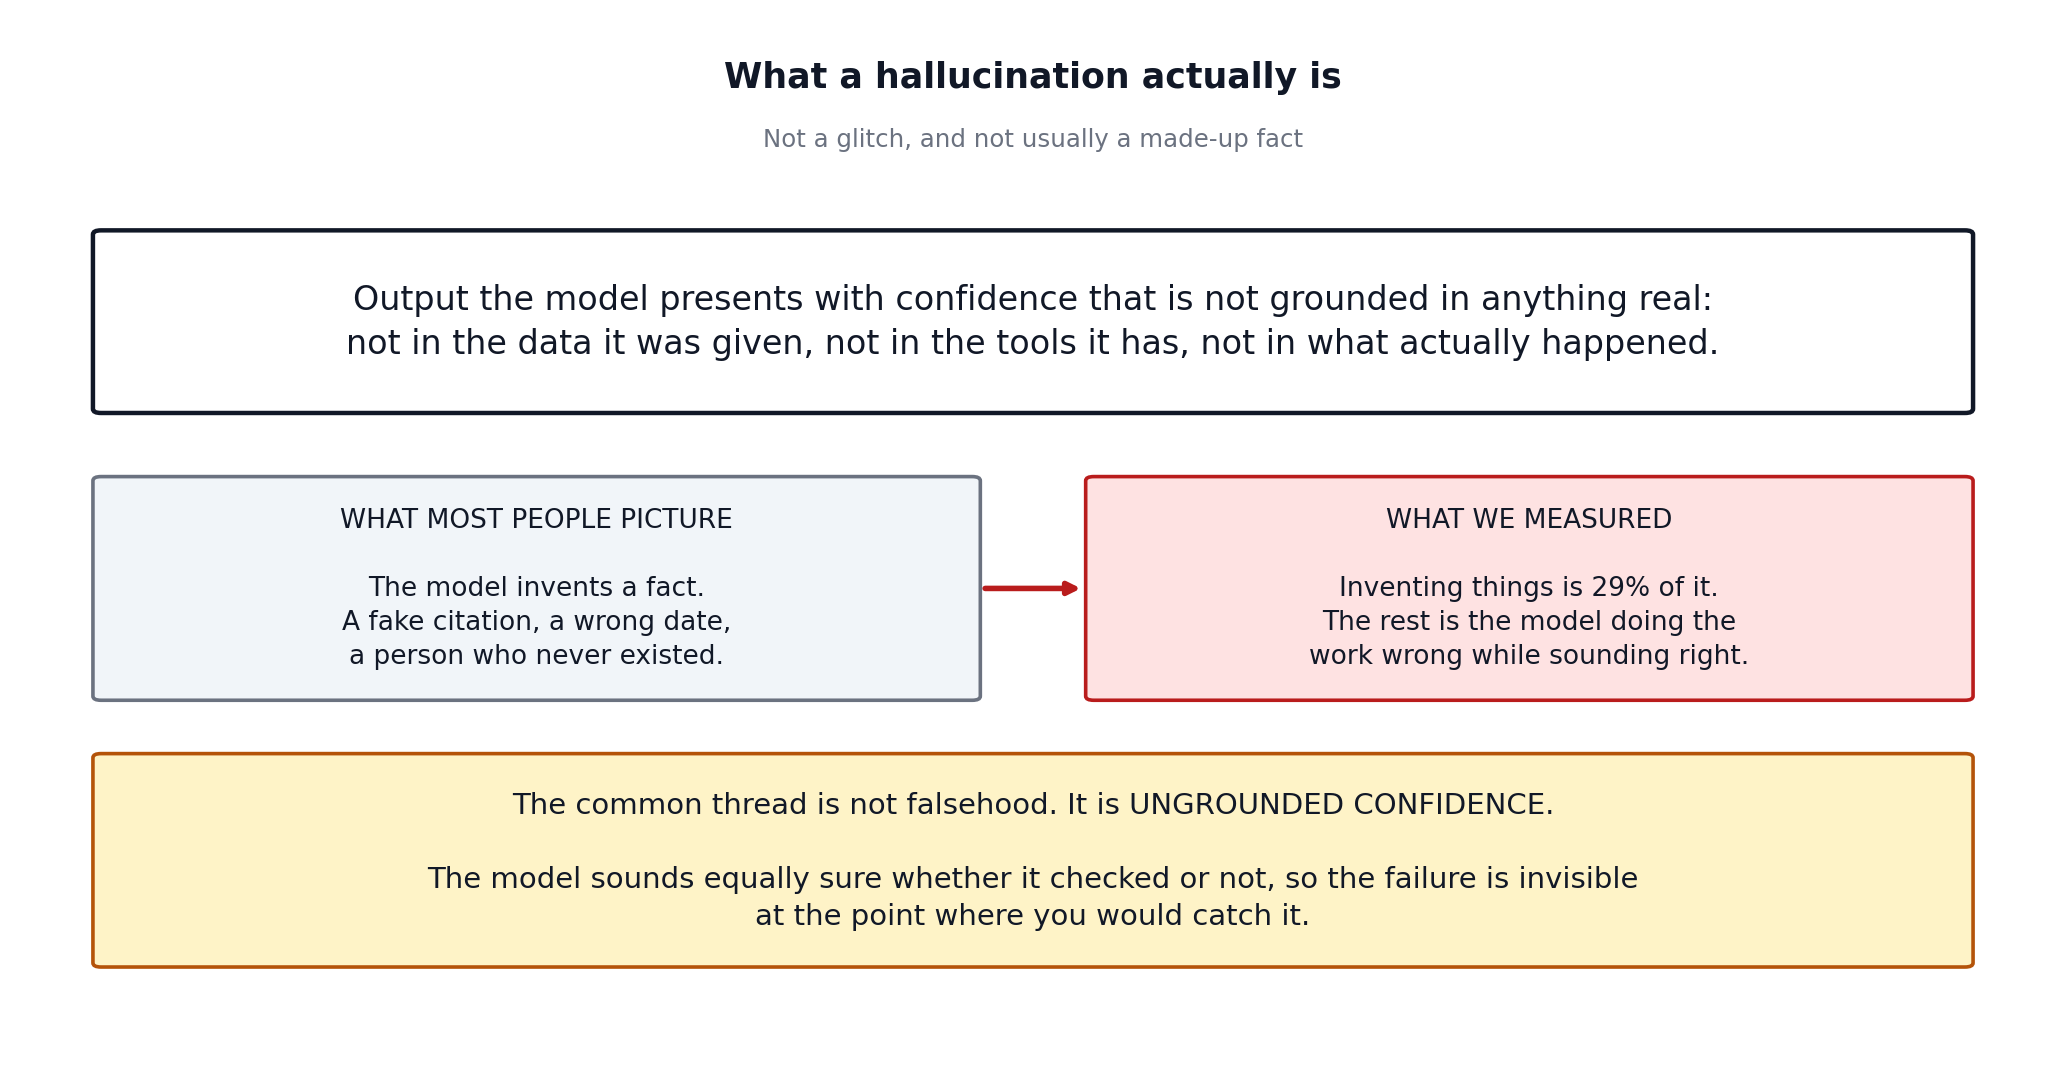
\includegraphics[width=\textwidth]{figures/fig1_what_is_a_hallucination.png}
\caption{The definition, and the gap between what the word usually means and
what we measured.}
\end{figure}

%======================================================================
\section{How these were found}

The taxonomy was not designed in advance and then looked for. It accumulated the
other way around.

An AI assistant worked on a long-running research project across hundreds of
sessions. Those sessions were recorded: every instruction, every tool call,
every file written, every correction the human made. When something went wrong,
it was named, defined, and added to a registry. Detection was then automated
where it could be, so the same failure could be counted rather than merely
remembered.

Three consequences of that method matter when reading the numbers.

\textbf{The counts are a floor, not a total.} They count failures that were
detected. A failure nobody noticed is not in here.

\textbf{The distribution reflects this kind of work.} These are sessions of
research engineering: writing code, querying data, deploying jobs. A customer
service assistant or a document summariser would show a different mix. The
classes are likely to generalise. The proportions are not.

\textbf{Naming came before measuring, and the gap is visible.} Six of the 51
types have been named and defined but not yet observed in the instrumented
record. They are kept in the taxonomy because a named failure with no
observations is a different thing from a failure that does not happen.

%======================================================================
\section{The eight classes}

\begin{figure}[H]
\centering
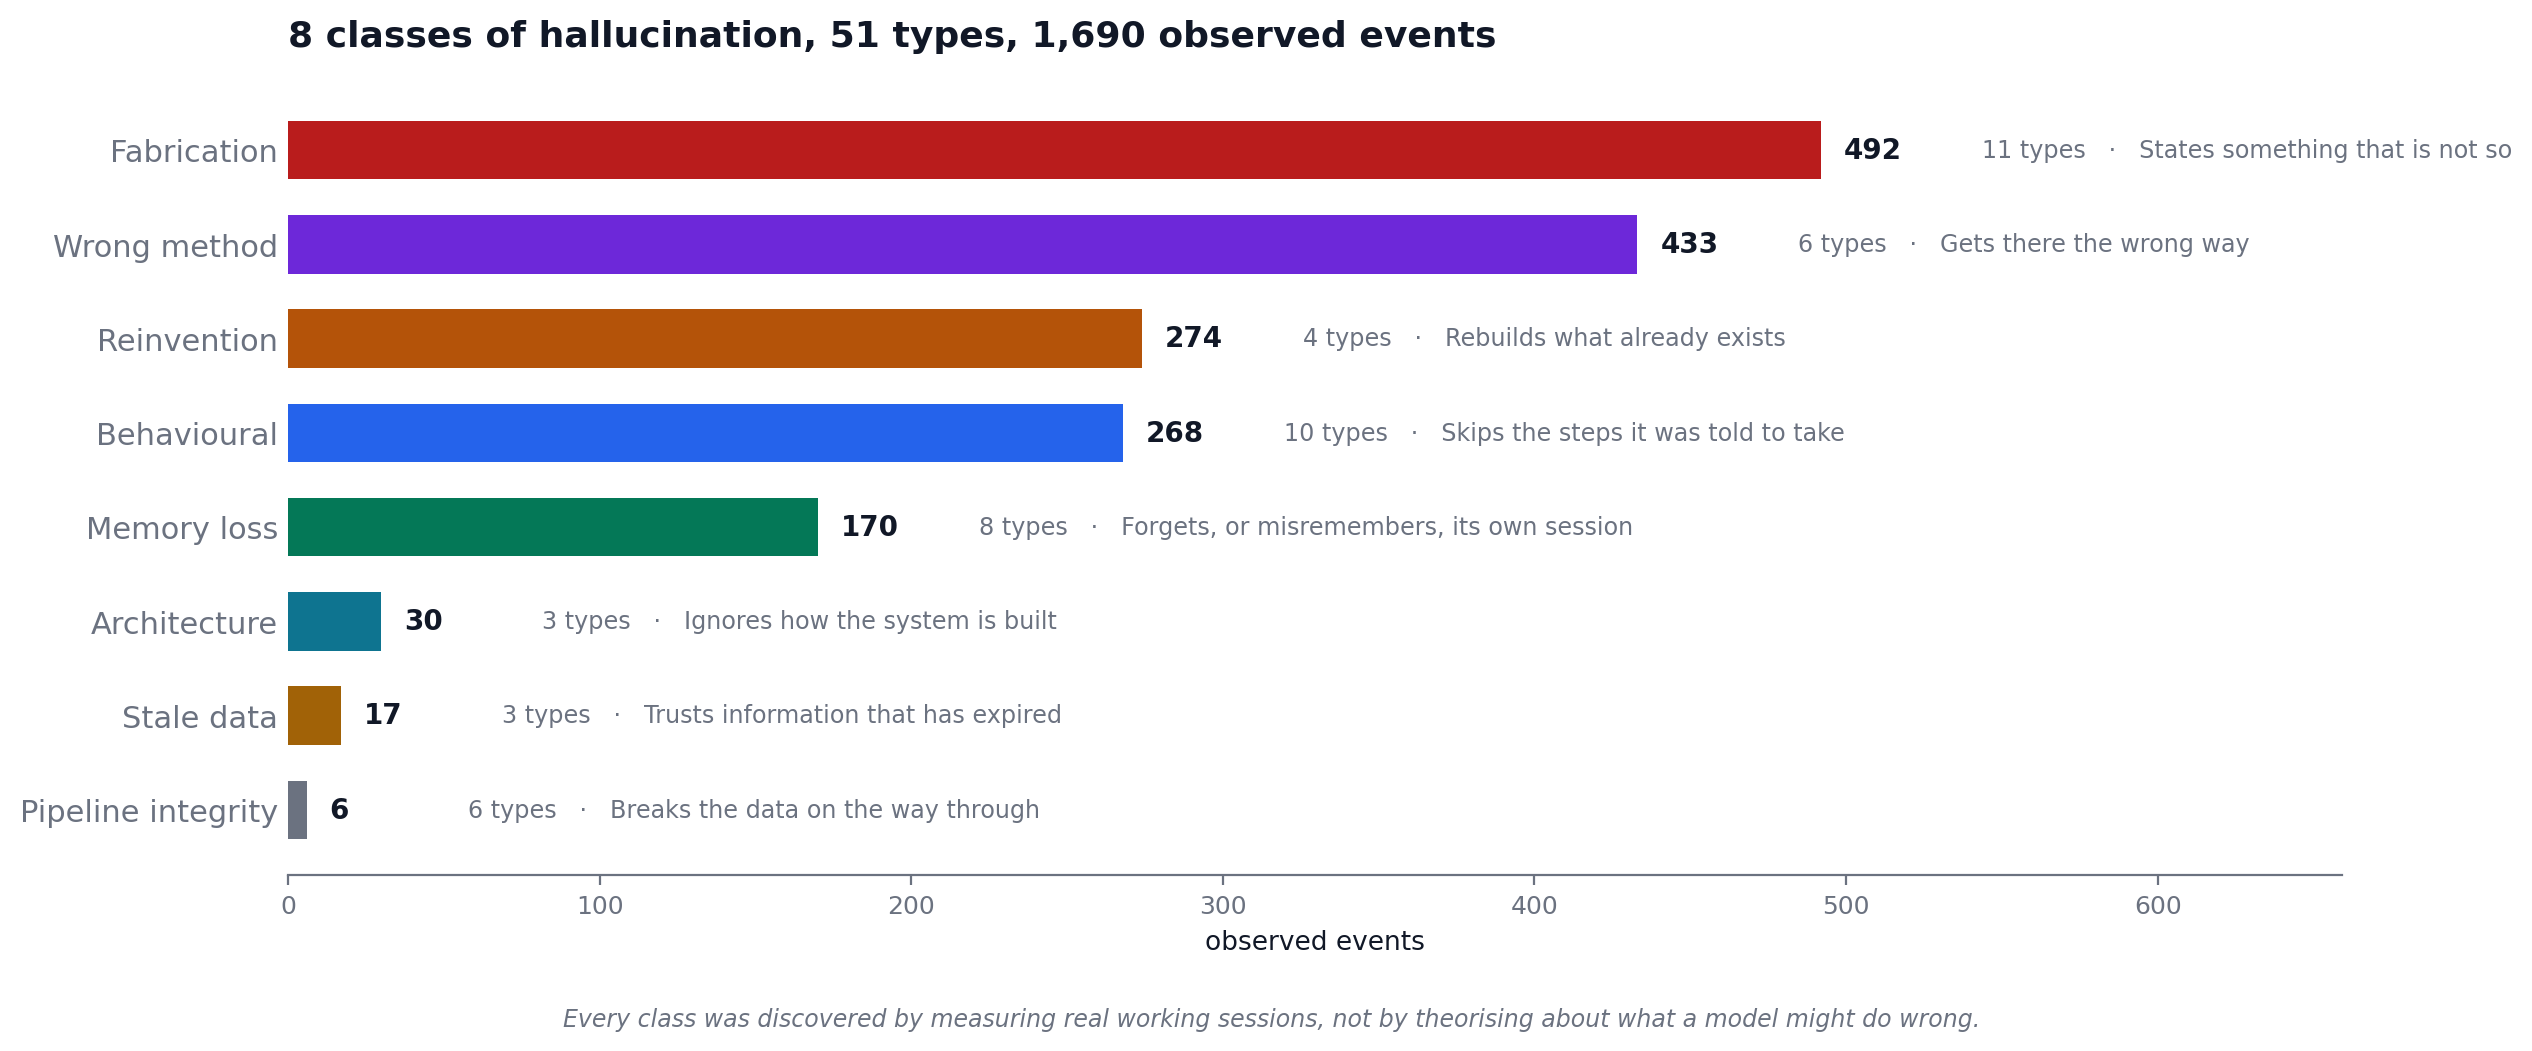
\includegraphics[width=\textwidth]{figures/fig2_eight_classes.png}
\caption{The eight classes, ordered by observed events. Fabrication leads, but
it is under a third of the total.}
\end{figure}

\begin{table}[H]
\centering
\small
\begin{tabular}{llrr}
\toprule
\textbf{Class} & \textbf{In one line} & \textbf{Types} & \textbf{Events} \\
\midrule
Fabrication         & States something that is not so           & 11 & 492 \\
Wrong method        & Gets there the wrong way                  & 6  & 433 \\
Reinvention         & Rebuilds what already exists              & 4  & 274 \\
Behavioural         & Skips the steps it was told to take       & 10 & 268 \\
Memory loss         & Forgets, or misremembers, its own session & 8  & 170 \\
Architecture        & Ignores how the system is built           & 3  & 30 \\
Stale data          & Trusts information that has expired       & 3  & 17 \\
Pipeline integrity  & Breaks the data on the way through        & 6  & 6 \\
\midrule
\textbf{Total}      &                                           & \textbf{51} & \textbf{1{,}690} \\
\bottomrule
\end{tabular}
\caption{The eight classes. ``Memory loss'' is called \texttt{compaction\_artifacts}
in the data: it covers what happens when a session runs long enough that the
model must compress its own history and loses things in the process.}
\end{table}

%======================================================================
\section{What the distribution says}

\begin{figure}[H]
\centering
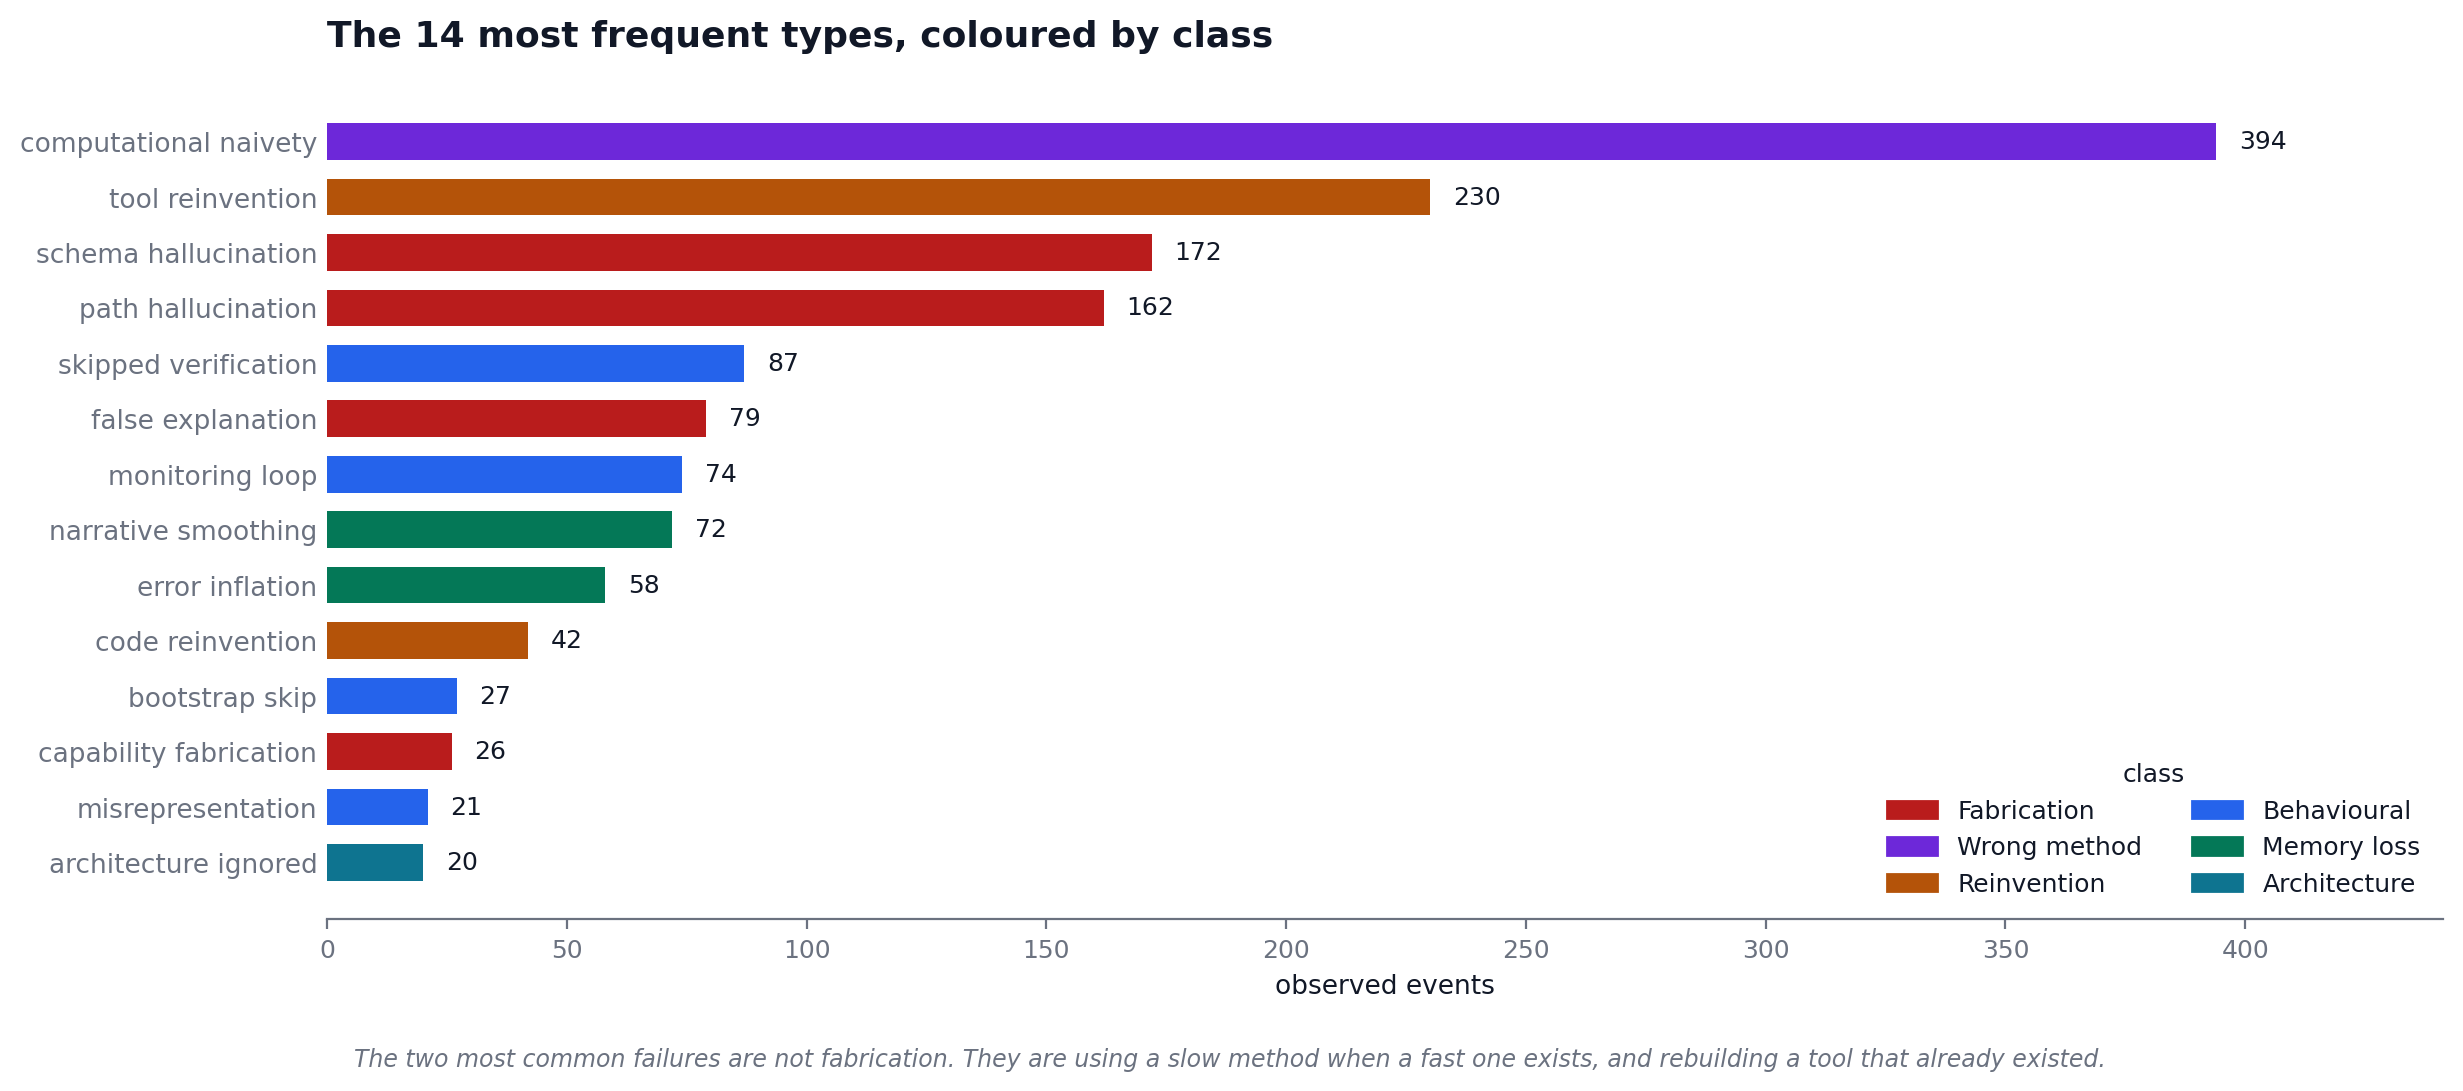
\includegraphics[width=\textwidth]{figures/fig3_type_breakout.png}
\caption{The sixteen most frequent types. The top two are not fabrication.}
\end{figure}

\textbf{Fabrication is 29\% of events.} It is the largest single class and it is
still under a third. A programme that addresses only fabrication addresses under
a third of the problem, while reporting that it has solved ``hallucination''.

\textbf{The single most common failure is a performance failure.}
\texttt{computational\_naivety}, 394 events, is the model writing a slow loop
when a fast bulk method was available. Nothing it produced was false. The work
was simply done the wrong way, at a cost nobody would see except in the clock.

\textbf{The second is a duplication failure.} \texttt{tool\_reinvention}, 230
events, is the model writing new code to do a job an existing tool already did.
The output usually works. It is still waste, and it still quietly grows the
amount of code somebody has to maintain.

\textbf{Two fabrication types dominate their class, and both are structural.}
\texttt{schema\_hallucination} (172 events) is querying a database using column
names that do not exist. \texttt{path\_hallucination} (162) is referring to files
that are not there. These are the two most confirmable failures in the whole
taxonomy, because a path either exists or it does not. That is why they carry
the highest structural confirmation counts, 164 and 155 respectively, and it
suggests something more general: the failures we can count best are the ones the
world can contradict directly.

%======================================================================
\section{How far each type has been taken}

\begin{figure}[H]
\centering
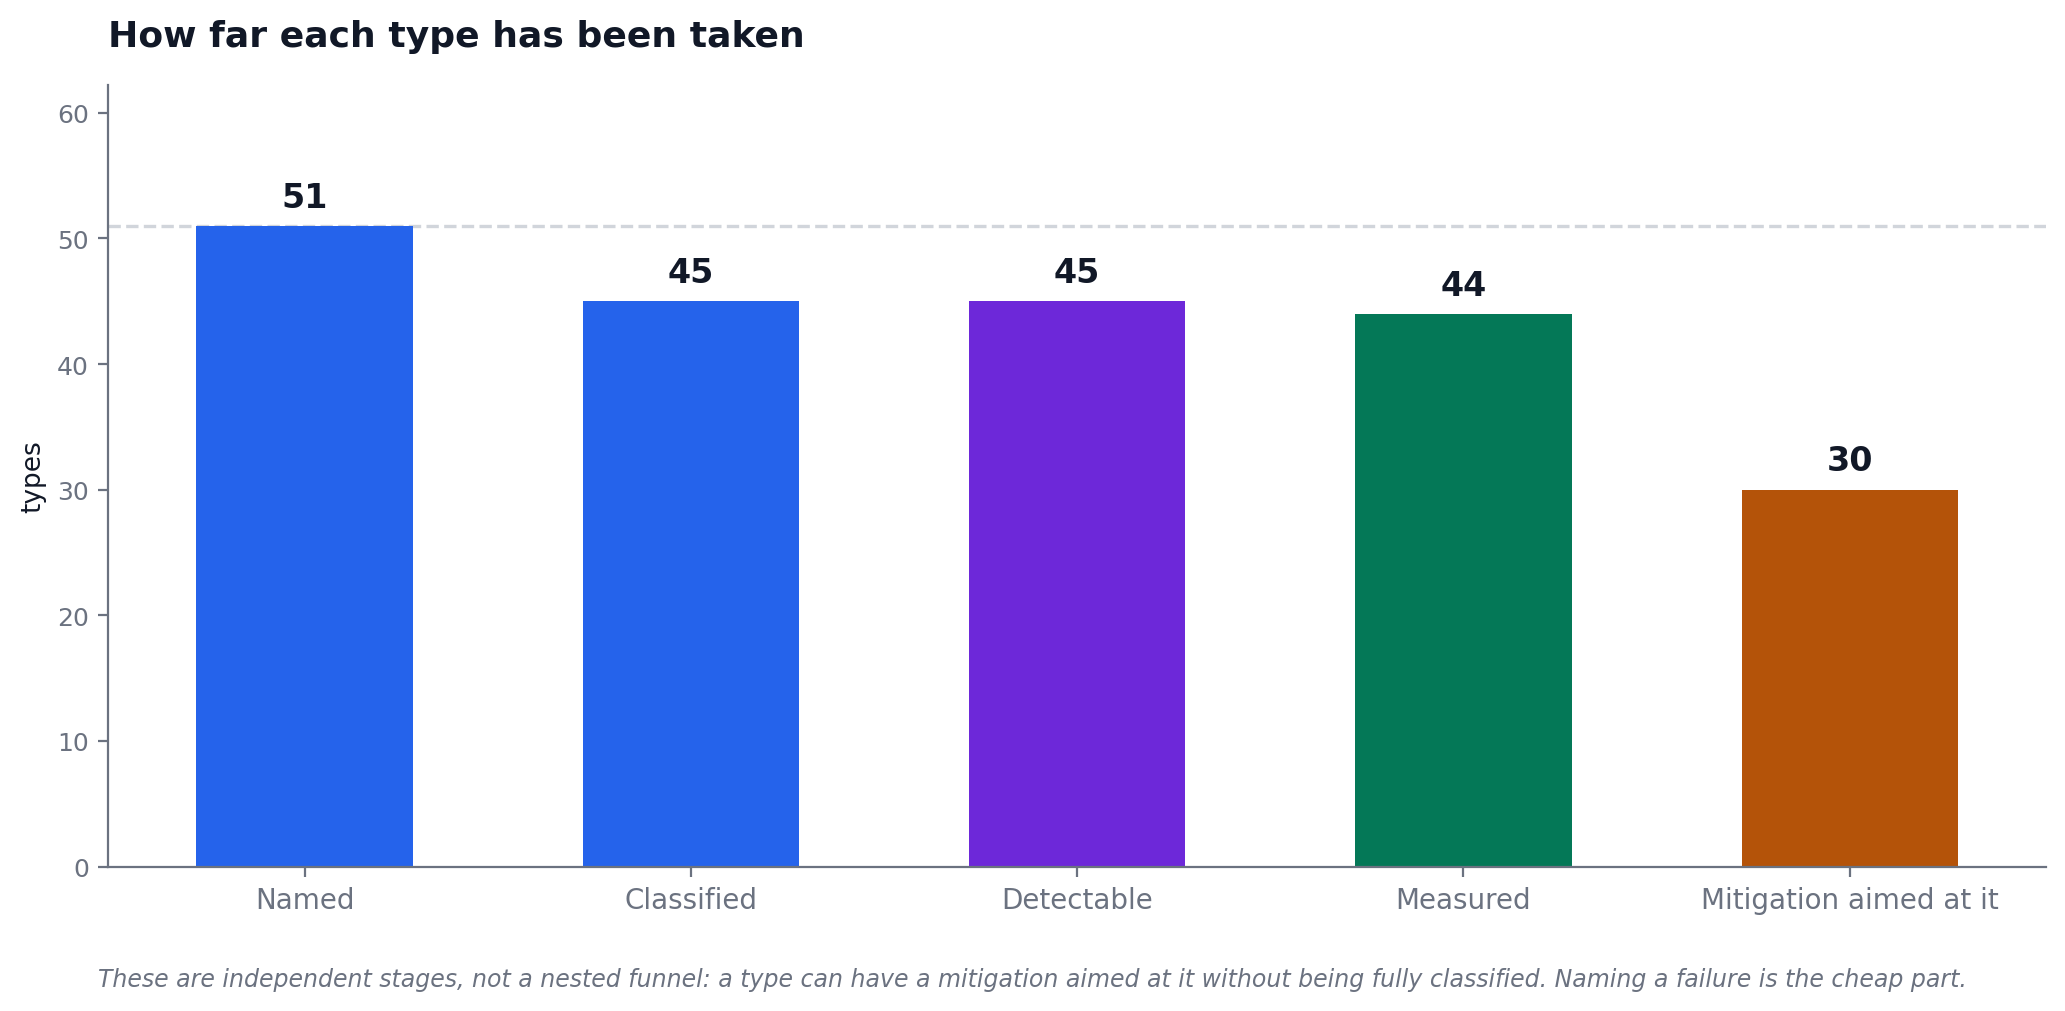
\includegraphics[width=\textwidth]{figures/fig4_coverage.png}
\caption{Naming a failure is the cheap part. These are independent stages rather
than a nested funnel: a type can have a mitigation aimed at it without being
fully classified.}
\end{figure}

All 51 types are named and defined. 45 are classified in the detection matrix,
44 have had their performance measured over time, and 30 have some mitigation
aimed specifically at them.

The gap between naming and mitigating is where the work actually stands. It is
straightforward to notice a failure and write down what it was. It is harder to
detect it automatically, harder again to design something that reduces it, and
hardest of all to show that the reduction is real rather than a lull.

%======================================================================
\section{The full list}

Every type, grouped by class, ordered by observed events within each class.

\small
\begin{longtable}{@{}p{0.30\textwidth}r p{0.60\textwidth}@{}}
\toprule
\textbf{Type} & \textbf{Events} & \textbf{What it is} \\
\midrule
\endhead
\multicolumn{3}{@{}l}{\textbf{FABRICATION} \quad 11 types, 492 events} \\
\midrule
schema\_hallucination & 172 & Queries a database using column or table names that do not exist \\
path\_hallucination & 162 & References file paths that do not exist, or writes to the wrong place \\
false\_explanation & 79 & Gives a confident causal explanation with no evidence behind it \\
capability\_fabrication & 26 & Claims a feature, tool, or API exists when it does not \\
capability\_overstatement & 13 & Plans actions it cannot actually perform in this environment \\
fabricated\_fact & 9 & Asserts a specific fact with no basis in the code or the runtime \\
gpu\_config\_hallucination & 8 & Misstates the hardware configuration. The most-repeated single error here \\
attribution\_misframing & 8 & Frames a structural gap as a personal oversight, implying agency it lacks \\
recurring\_false\_belief & 7 & Repeats a false claim after being corrected \\
defensive\_fabrication & 7 & Invents a constraint to avoid admitting it must backtrack \\
rationalized\_observation & 1 & Explains an accidental state as though it were deliberate design \\
\midrule
\multicolumn{3}{@{}l}{\textbf{WRONG METHOD} \quad 6 types, 433 events} \\
\midrule
computational\_naivety & 394 & Uses a slow loop when a fast bulk method exists \\
redundant\_recomputation & 17 & Recomputes from scratch when the answer was already cached \\
deployment\_sequence\_error & 8 & Runs deployment steps out of order, or mishandles a stuck state \\
agent\_prompt\_underspecification & 6 & Tells a sub-agent the task but not the context, so it falls back to defaults \\
serial\_when\_parallel & 5 & Runs on one core or one GPU when many were available \\
search\_scope\_narrowing & 3 & Searches where it expects things to be and misses the obvious place \\
\midrule
\multicolumn{3}{@{}l}{\textbf{REINVENTION} \quad 4 types, 274 events} \\
\midrule
tool\_reinvention & 230 & Ignores an available tool and writes ad-hoc code instead \\
code\_reinvention & 42 & Writes new code for something the codebase already does \\
foundational\_rederivation & 2 & Rebuilds an authoritative artifact from scratch rather than fixing one row \\
infrastructure\_reinvention & 0 & Rebuilds infrastructure that already exists \\
\midrule
\multicolumn{3}{@{}l}{\textbf{BEHAVIOURAL} \quad 10 types, 268 events} \\
\midrule
skipped\_verification & 87 & Proceeds to full execution without checking intermediate results \\
monitoring\_loop & 74 & Blocks the session polling or sleeping in a loop \\
bootstrap\_skip & 27 & Starts work without the mandatory session setup, cascading failures later \\
misrepresentation & 21 & Says work is done or working when it is partial or untested \\
unwarranted\_confidence & 17 & Asserts a fact without verifying it, and is wrong \\
unsolicited\_development & 13 & Builds a full implementation without asking first \\
scope\_inflation & 13 & Expands the job beyond what was asked \\
exuberance & 6 & Writes far more code than requested \\
tool\_preference\_persistence & 6 & Reverts to a familiar tool after being corrected three or more times \\
cross\_session\_amnesia & 4 & Repeats an approach that already failed in an earlier session \\
\midrule
\multicolumn{3}{@{}l}{\textbf{MEMORY LOSS} \quad 8 types, 170 events} \\
\midrule
narrative\_smoothing & 72 & Summarises its own session as tidier and more sequential than it was \\
error\_inflation & 58 & Misreports successful operations as errors when summarising \\
compression\_artifact & 14 & Compresses distinct items into ``repeated'' or ``similar'', losing the distinction \\
post\_compaction\_amnesia & 9 & Keeps the gist after compressing history but loses the operational detail \\
message\_dropping & 9 & Omits a user instruction entirely from its summary \\
attribute\_substitution & 6 & Identifies the right thing but attaches the wrong properties to it \\
context\_rotation\_drift & 2 & Drifts further from the original intent with each successive summary \\
attribution\_drift & 0 & Attaches a real fact to the wrong entity \\
\midrule
\multicolumn{3}{@{}l}{\textbf{ARCHITECTURE} \quad 3 types, 30 events} \\
\midrule
architecture\_ignored & 20 & Knew the established pattern and violated it anyway \\
architecture\_unknown & 7 & Designed something without knowing the existing architecture \\
architecture\_reinvented & 3 & Duplicated an existing design decision one level up \\
\midrule
\multicolumn{3}{@{}l}{\textbf{STALE DATA} \quad 3 types, 17 events} \\
\midrule
stale\_ephemeral\_state & 10 & Assumed a process or hardware state was still current \\
stale\_data\_citation & 4 & Cited an out-of-date source as though it were current \\
stale\_data\_no\_freshness & 3 & Did not check how old the data was before citing it \\
\midrule
\multicolumn{3}{@{}l}{\textbf{PIPELINE INTEGRITY} \quad 6 types, 6 events} \\
\midrule
index\_misalignment & 5 & Joined data sources that use incompatible identifiers \\
label\_miscount & 1 & Assumed the wrong number of classes in a dataset \\
truncation\_loss & 0 & An infrastructure bug silently destroyed content \\
circular\_validation & 0 & A check consumes the labels it was supposed to verify, so it always passes \\
dedup\_collision & 0 & A key design error silently dropped rows during deduplication \\
stitched\_spaces & 0 & Combined outputs from models that are not comparable \\
\bottomrule
\end{longtable}
\normalsize

%======================================================================
\section{What this does not show}

\textbf{One project, one kind of work.} These sessions are research engineering.
The proportions would look different for a chatbot, a summariser, or a coding
assistant used a different way. Treat the classes as portable and the percentages
as local.

\textbf{Detected, not total.} Every count is a floor. The types with the highest
confirmation counts are the ones reality can contradict most directly, which
means the taxonomy is better at counting checkable failures than subtle ones. A
low number can mean a rare failure or a hard-to-see one, and this table does not
distinguish them.

\textbf{Counts depend on which record you use.} The figure of 1,690 is the
observed-event count in the detection matrix. Other counts in the same system
answer slightly different questions and give different totals. Any single number
quoted from this work should name the record it came from.

\textbf{Two internal records disagree on the type list.} A curated registry holds
31 types; the inventory used here holds 51. The 20-type difference includes the
two largest fabrication types. This document uses the inventory. Reconciling the
two is open work.

%======================================================================
\section{Where a deeper discussion would go}

Four questions this orientation raises and does not answer.

\begin{enumerate}
  \item \textbf{Does naming a failure reduce it?} The record includes the dates
        a type was named and the dates mitigations were introduced, so this is
        measurable rather than a matter of opinion. Some types were suppressed
        after mitigation. Others recurred regardless.
  \item \textbf{Which failures are worth mitigating?} A type with 394 events that
        costs a few seconds each may matter less than a type with 7 events that
        silently corrupts a result.
  \item \textbf{Can a model detect its own hallucinations in flight?} Detecting
        them after the fact in a transcript is a solved problem for several of
        these types. Catching them at the moment of production is not.
  \item \textbf{How much transfers?} The eight classes come from one project.
        Whether they cover generative AI failure generally is an empirical
        question nobody has run.
\end{enumerate}

\end{document}
